\iffalse
\documentclass[journal,12pt,twocolumn]{IEEEtran}
\usepackage{setspace}
\usepackage{gensymb}
\usepackage{xcolor}
\usepackage{caption}
\singlespacing
\usepackage{siunitx}
\usepackage[cmex10]{amsmath}
\usepackage{mathtools}
\usepackage{hyperref}
\usepackage{amsthm}
\usepackage{mathrsfs}
\usepackage{txfonts}
\usepackage{stfloats}
\usepackage{cite}
\usepackage{cases}
\usepackage{subfig}
\usepackage{longtable}
\usepackage{multirow}
\usepackage{enumitem}
\usepackage{bm}
\usepackage{mathtools}
\usepackage{listings}
\usepackage{tikz}
\usetikzlibrary{shapes,arrows,positioning}
\usepackage{circuitikz}
\renewcommand{\vec}[1]{\boldsymbol{\mathbf{#1}}}
\DeclareMathOperator*{\Res}{Res}
\renewcommand\thesection{\arabic{section}}
\renewcommand\thesubsection{\thesection.\arabic{subsection}}
\renewcommand\thesubsubsection{\thesubsection.\arabic{subsubsection}}

\renewcommand\thesectiondis{\arabic{section}}
\renewcommand\thesubsectiondis{\thesectiondis.\arabic{subsection}}
\renewcommand\thesubsubsectiondis{\thesubsectiondis.\arabic{subsubsection}}
\hyphenation{op-tical net-works semi-conduc-tor}

\lstset{
language=Python,
frame=single, 
breaklines=true,
columns=fullflexible
}
\begin{document}
\theoremstyle{definition}
\newtheorem{theorem}{Theorem}[section]
\newtheorem{problem}{Problem}
\newtheorem{proposition}{Proposition}[section]
\newtheorem{lemma}{Lemma}[section]
\newtheorem{corollary}[theorem]{Corollary}
\newtheorem{example}{Example}[section]
\newtheorem{definition}{Definition}[section]
\newcommand{\BEQA}{\begin{eqnarray}}
        \newcommand{\EEQA}{\end{eqnarray}}
\newcommand{\define}{\stackrel{\triangle}{=}}
\newcommand{\myvec}[1]{\ensuremath{\begin{pmatrix}#1\end{pmatrix}}}
\newcommand{\mydet}[1]{\ensuremath{\begin{vmatrix}#1\end{vmatrix}}}
\bibliographystyle{IEEEtran}
\providecommand{\nCr}[2]{\,^{#1}C_{#2}} % nCr
\providecommand{\nPr}[2]{\,^{#1}P_{#2}} % nPr
\providecommand{\mbf}{\mathbf}
\providecommand{\pr}[1]{\ensuremath{\Pr\left(#1\right)}}
\providecommand{\qfunc}[1]{\ensuremath{Q\left(#1\right)}}
\providecommand{\sbrak}[1]{\ensuremath{{}\left[#1\right]}}
\providecommand{\lsbrak}[1]{\ensuremath{{}\left[#1\right.}}
\providecommand{\rsbrak}[1]{\ensuremath{{}\left.#1\right]}}
\providecommand{\brak}[1]{\ensuremath{\left(#1\right)}}
\providecommand{\lbrak}[1]{\ensuremath{\left(#1\right.}}
\providecommand{\rbrak}[1]{\ensuremath{\left.#1\right)}}
\providecommand{\cbrak}[1]{\ensuremath{\left\{#1\right\}}}
\providecommand{\lcbrak}[1]{\ensuremath{\left\{#1\right.}}
\providecommand{\rcbrak}[1]{\ensuremath{\left.#1\right\}}}
\theoremstyle{remark}
\newtheorem{rem}{Remark}
\newcommand{\sgn}{\mathop{\mathrm{sgn}}}
\newcommand{\rect}{\mathop{\mathrm{rect}}}
\newcommand{\sinc}{\mathop{\mathrm{sinc}}}
\providecommand{\abs}[1]{\left\vert#1\right\vert}
\providecommand{\res}[1]{\Res\displaylimits_{#1}}
\providecommand{\norm}[1]{\lVert#1\rVert}
\providecommand{\mtx}[1]{\mathbf{#1}}
\providecommand{\mean}[1]{E\left[ #1 \right]}
\providecommand{\fourier}{\overset{\mathcal{F}}{ \rightleftharpoons}}
\providecommand{\ztrans}{\overset{\mathcal{Z}}{ \rightleftharpoons}}
\providecommand{\system}[1]{\overset{\mathcal{#1}}{ \longleftrightarrow}}
\newcommand{\solution}{\noindent \textbf{Solution: }}
\providecommand{\dec}[2]{\ensuremath{\overset{#1}{\underset{#2}{\gtrless}}}}
\let\StandardTheFigure\thefigure
\def\putbox#1#2#3{\makebox[0in][l]{\makebox[#1][l]{}\raisebox{\baselineskip}[0in][0in]{\raisebox{#2}[0in][0in]{#3}}}}
\def\rightbox#1{\makebox[0in][r]{#1}}
\def\centbox#1{\makebox[0in]{#1}}
\def\topbox#1{\raisebox{-\baselineskip}[0in][0in]{#1}}
\def\midbox#1{\raisebox{-0.5\baselineskip}[0in][0in]{#1}}

\vspace{3cm}
\title{11.11.4.5}
\author{Lokesh Surana}
\maketitle
\section*{Class 11, Chapter 11, Exercise 4.5}
\fi
The equation of the hyperbola can be rearranged as
\begin{align}
	\label{eq:chapters/11/11/4/5/1}
	-x^2 + \frac{5}{9}y^2 -4 = 0
\end{align}
The above equation can be equaded to the generic equation of conic sections
\begin{align}
	\label{eq:chapters/11/11/4/5/2}
	g\brak{\vec{x}}=\vec{x}^\top \vec{V} \vec{x} + 2\vec{u}^\top \vec{x} + f = 0
\end{align}
Comparing coefficients of both equations \eqref{eq:chapters/11/11/4/5/1} and \eqref{eq:chapters/11/11/4/5/2}
\begin{align}
	\label{3}
	\vec{V} &= \myvec{-1&0\\0&\frac{5}{9}}\\
	\vec{u} &= \vec{0}\\
	f &= -4
\end{align}

From equation \eqref{3}, since $\vec{V}$ is already diagonalized, the eigen values $\lambda_1 \text{ and } \lambda_2$ are given as
\begin{align}
	\lambda_1 &= -1\\
	\lambda_2 &= \frac{5}{9}
\end{align}
\begin{enumerate}
\item The eccentricity of the hyperbola is given as
\begin{align}
	e &= \sqrt{1 - \frac{\lambda_2}{\lambda_1}} = \sqrt{1+\frac{5}{9}}\\
	  &= \frac{\sqrt{14}}{3}
\end{align}
\item For the standard hyperbola, the coordinates of Focii are given as
\begin{align}
	\label{eq:chapters/11/11/4/5/4}
	\vec{F} = \pm \frac{\brak{\frac{1}{e\sqrt{1-e^2}}}\brak{e^2}\sqrt{\frac{\lambda_1}{f_0}}}{\frac{\lambda_1}{f_0}} \vec{e}_2
\end{align}
where
\begin{align}
	f_0 &= -f\\
	\eqref{eq:chapters/11/11/4/5/4} \implies &= \pm \frac{\brak{\frac{1}{\frac{\sqrt{14}}{3}\sqrt{1-\frac{14}{9}}}}\brak{\frac{14}{9}}\sqrt{\frac{-1}{4}}}{\frac{-1}{4}} \vec{e}_2\\
	&= \pm \myvec{0\\\frac{6}{2\sqrt{\frac{14}{5}}}}
\end{align}
\item The vertices of the hyperbola are given by
\begin{align}
	\pm \myvec{0\\\sqrt{\abs{\frac{f_0}{\lambda_2}}}}= \pm \myvec{0\\\frac{6}{\sqrt{5}}}
\end{align}
\item The length of latus rectum is given as
\begin{align}
	2\frac{\sqrt{\abs{f_0 \lambda_2}}}{\lambda_1} &= 2\frac{\sqrt{\abs{14\brak{\frac{5}{9}}}}}{-1}\\
	&= 4\frac{\sqrt{5}}{3}
\end{align}
as length cannot be negative.
\end{enumerate}

\begin{figure}[!h]
	\begin{center} 
	    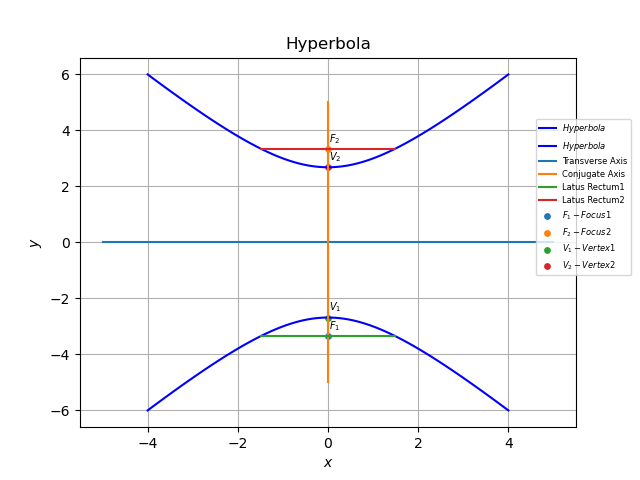
\includegraphics[width=\columnwidth]{chapters/11/11/4/5/figs/hyperbola.png}
	\end{center}
\caption{}
\label{fig:chapters/11/11/4/5/1}
\end{figure}

